\chapter{全局通用技术}

\begin{lemma}
\begin{multline*}
	f, g \mbox{在} x_0 \mbox{有公共切线} \\ \Rightarrow f(x_0) = g(x_0), f'(x_0) = g'(x_0)
\end{multline*}
\end{lemma}
上述内容中小心遗漏 $f(x_0) = g(x_0)$

\begin{definition}
    \begin{equation}
        \mathbf{C}_{k}^{n} = \binom{n}{k} = \frac{n!}{k!(n-k)!}
    \end{equation}
\end{definition}

\begin{lemma}
    \begin{align*}
        (a+b)^3 = a^3 + 3a^2b + 3ab^2 + b^3\\
        (a-b)^3 = a^3 - 3a^2b + 3ab^2 - b^3
    \end{align*}
\end{lemma}

\section{函数}

无论是导数还是积分,相关题目和函数性质(图像、单调性等)相关性总是很大,
在处理的时候要善于利用函数的性质,辅助解题。
利用函数性质辅助解题的有例子:
题目 
\begin{itemize}

    \item   \cite[page 70, pdf 81, 例1]{we} 和 
            \cite[page 75, pdf 86, 例6]{we}利用函数是偶函数,
            因此图像对称,从而你确定第二条渐近线。

    \item   题目 \cite[page 77, pdf 88, 例5, 例6]{we} 
            通过观察函数图像,辅助确定根的个数,
            有关根的个数请参阅 \ref{number-of-roots-question}。

    \item   题目 \cite[page 107, pdf 118, example 4]{we}
            认识到原函数是偶函数,进而简化求值过程。

\end{itemize}

\subsection{如何联系函数和导数}

TODO
%TODO

\section{Tylor Series and Formula} \label{tylor}

\subsection{公式和形式}

\begin{definition}[泰勒公式的一般形式]
	\begin{equation}
		f(x)=\sum_{i=0}^{n}{\frac{f^{(i)}(x_0)}{i!}(x-x_0)^i}+R_n(x)
	\end{equation}
	其中,$f^{(i)}(x_0)$表示$f(x)$在$x_0$处的$i$阶导数,$R_n(x)$表示余项,有多种形式,例如:
	\begin{align*}
		&R_n(x)=\frac{f^{(n+1)}(\xi)}{(n+1)!}(x-x_0)^{n+1}, \\ &\xi \in [x,x_0]\ or \ \xi \in [x_0,x]
	\end{align*}
\end{definition}

In summary, the Peano remainder focuses on 
the local behavior of the function near the point of expansion 
and gives a rough upper bound on the error for a specific value of $x$. 
\begin{definition}{The Cauchy remainder}
    \[
        R_n=\dfrac{(x-x^*)^n}{n!}(x-x_0)f^{(n+1)}(x^*)
    \]
    where $x^*$ is in $[x_0,x]$ (Hamilton 1952).
\end{definition}
The \textbf{Cauchy remainder provides a more global perspective by 
considering the behavior of derivatives across a broader 
interval between $x_0$ and $x$}. It gives a more refined estimate 
of the error over that interval. This distinction in the scope 
of accuracy makes the Cauchy remainder more useful when you want 
to understand how well the Taylor polynomial approximates the function 
across a larger range of values.

下面是常用的一些Tylor公式
\begin{align}
    \label{eq:useful-tylor-expandations}
	\notag e^x&=1+x+\frac{x^2}{2!}+\frac{x^3}{3!} \\ &+\cdots+\frac{x^n}{n!}+o(x^n)\\
	\notag \ln(1+x)&=x-\frac{x^2}{2}+\frac{x^3}{3}\\ &-\cdots+(-1)^{n-1}\frac{x^n}{n}+o(x^n)\\
	\notag \sin x&=x-\frac{x^3}{3!}+\frac{x^5}{5!}\\ &-\cdots+(-1)^{n-1}\frac{x^{2n-1}}{(2n-1)!}+o(x^{2n})\\
	\notag \cos x&=1-\frac{x^2}{2!}+\frac{x^4}{4!}\\ &-\cdots+(-1)^n\frac{x^{2n}}{(2n)!}+o(x^{2n+1})\\
           \tan x&=x+\frac{1}{3}x^3 + \frac{2}{15}x^5 + \frac{7}{315}x^7 + o(x^7)\\
           \arcsin x&= x + \frac{1}{6} x^3 + o(x^3) \\
           \arctan x&= x - \frac{1}{3} x^3 + o(x^3) \\
	\notag (1+x)^\alpha&=1+\alpha x+\frac{\alpha(\alpha-1)}{2!}x^2+ \\  &\cdots+\frac{\alpha(\alpha-1)\cdots(\alpha-n+1)}{n!}x^n+o(x^n)
\end{align}

等价无穷小\footnote{参见小节\ref{super-small}}就是化简的Tylor展开替换。
在使用的时候可以结合对应的Tylor公式来保证替换的正确性。

\subsection{做题应用} \label{tylor-app}

其中,\textbf{奇函数}的麦克劳林级数展开中偶数阶导数系数为0。

\section{不等式} \label{inequlity}

\subsection{随听课新增的}

\begin{lemma}
    \begin{gather*}
        \dfrac{x}{1+x} < \ln (1+x) < x \\
        2ab \leq a^2 + b^2 \\
        |x\pm y| \leq |x| \pm |y| \\
        e^x \leq 1 + x
    \end{gather*}
\end{lemma}
如图 \ref{fig:x-slash-1-plus-x-ln-x-x},
辅助记忆不等式的同时,
但也请注意他们在 $0$ 点处的特性。

\begin{figure}
  \centering
  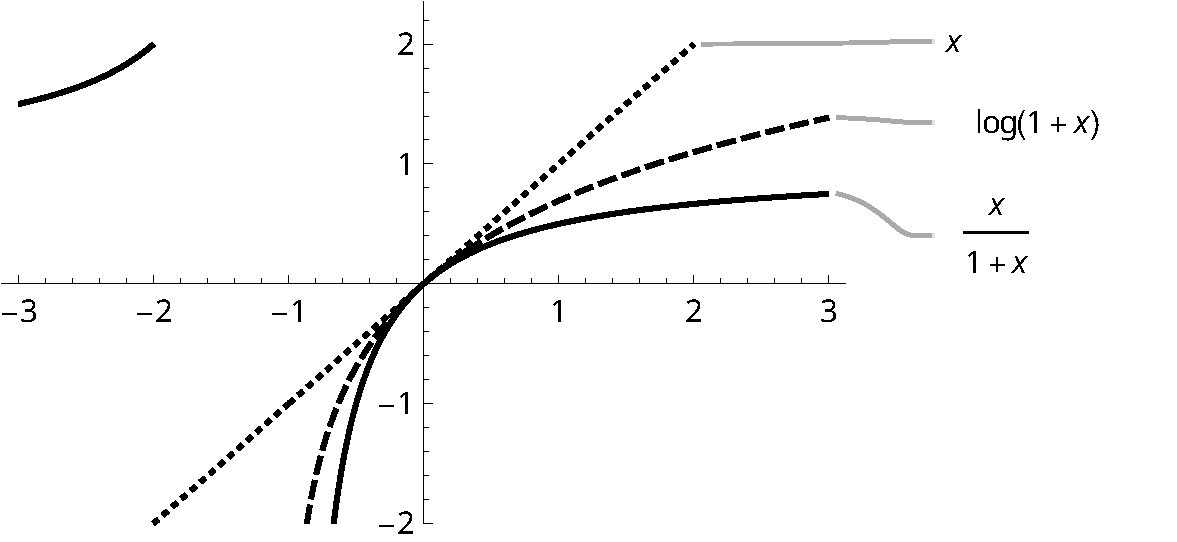
\includegraphics[width=0.55\textwidth]{figure/x-slash-1-plus-x-ln-x-x.pdf}
  \caption{The figure of $x/(1+x), \ln{(1+x)}, x$.}
  \label{fig:x-slash-1-plus-x-ln-x-x}
\end{figure}

\subsection{基本不等式}

考研数学中常用的不等式有以下几类:

对非负实数$a,b$,有
\begin{equation}
	a+b \geq 2\sqrt {ab}
\end{equation}
等号成立当且仅当$a=b$.

对正实数$a,b$,有
\begin{equation}
	\dfrac{a}{b}+\dfrac{b}{a} \geq 2
\end{equation}
等号成立当且仅当$a=b$.

对任意实数$x,y$,有
\begin{equation}
	(x+y)^2 \leq 2(x^2+y^2)
\end{equation}
等号成立当且仅当$x=y$或$x=-y$.

对任意实数$x,y,z$,有
\begin{equation}
	(x+y+z)^2 \leq 3(x^2+y^2+z^2)
\end{equation}
等号成立当且仅当$x=y=z$.

对任意实数$x_1,x_2,\dots,x_n$和正整数$n$,有
\begin{equation}
	\dfrac{x_1+x_2+\cdots+x_n}{n} \geq \sqrt[n]{x_1x_2\cdots x_n}
\end{equation}
等号成立当且仅当$x_1=x_2=\cdots=x_n$.

对任意实数$a,b,c$和正整数$n$,有
\begin{equation}
	(a^n+b^n+c^n)^3 \geq 27a^nb^nc^n(a+b+c)^n
\end{equation}
等号成立当且仅当$a=b=c$.

对任意实数$a,b,c,d$和正整数$n,m$,有
\begin{equation}
	\begin{array}{c}
		(a^n+b^n+c^n+d^n)(a^m+b^m+c^m+d^m)\\ \geq \\(a^{n+m}+b^{n+m}+c^{n+m}+d^{n+m})^2
	\end{array}
\end{equation}
等号成立当且仅当$a=b=c=d$.

\subsection{三角不等式}
考研数学中常用的三角不等式有以下几种:

\subsubsection{绝对值形式}
对任意实数$a,b$,有
\begin{equation}
	|a-b| \leq |a|+|b|
\end{equation}
等号成立当且仅当$a,b$同号或其中一个为零.

对任意实数$a,b,c$,有
\begin{equation}
	|a+b+c| \leq |a|+|b|+|c|
\end{equation}
等号成立当且仅当$a,b,c$同号或其中两个为零.

对任意实数$a_1,a_2,\dots,a_n$和正整数$n$,有
\begin{equation}
	|a_1+a_2+\cdots+a_n| \leq |a_1|+|a_2|+\cdots+|a_n|
\end{equation}
等号成立当且仅当$a_1,a_2,\dots,a_n$同号或其中$n-1$个为零.

\subsubsection{向量形式}
对$n$维向量 
$\pmb{x}=(x_1,x_2,\dots,x_n),$
$\pmb{y}=(y_1,y_2,\dots,y_n)$,有
\begin{equation}
	|\pmb{x}|-|\pmb{y}|\leqslant |\pmb{x}\pm\pmb{y}|\leqslant |\pmb{x}|+|\pmb{y}|
\end{equation}
等号成立当且仅当$\pmb{x}\parallel\pmb{y}$.

对$n$维向量$\pmb{x}=(x_1,x_2,\dots,x_n),\pmb{y}=(y_1,y_2,\dots,y_n),$
$\pmb{z}=(z_1,z_2,\dots,z_n)$,有
\begin{equation}
	|\pmb{x}+\pmb{y}+\pmb{z}| \leq |\pmb{x}|+|\pmb{y}|+|\pmb{z}|
\end{equation}

\section{巨算符} \label{giant-operator}

\cite[page A36]{stewart}
\[
    \sum \dfrac{f(x)}{g(x)} \neq \dfrac{\sum f(x)}{\sum g(x)}
\]

\section{对数}\label{logrithemic}

\begin{theorem}
    \begin{gather*}
        \log_a (mn) = \log_a m + \log_a n \\
        \log_a \left(\dfrac{m}{n}\right) = \log_a m - \log_a n \\
        \log_a \left(m^n\right) = n \log_a m  \\
        \log_a \left(\sqrt[n]{m}\right) = \dfrac{1}{n} \log_a m
    \end{gather*}
\end{theorem}

在使用对数函数的时候,必要的时候不要忘记标注定义域。如
\cite[page 76, pdf 87, example 2]{we}.

\section{三角函数相关} \label{trigonometric}

\begin{corollary}
    \begin{equation}
        \arctan x + \arctan \dfrac{1}{x} = \dfrac{\pi}{2} \quad (x > 0)
    \end{equation}
\end{corollary}

\begin{corollary}
    \begin{align}
        \cos(\sin x) - \cos x &=    2 \sin \dfrac{x + \sin x}{2} \sin \dfrac{x- \sin x}{2} \label{eq:fucking-socalled-trig-formula} \\
        \cos(\sin x) - \cos x &\sim \dfrac{1}{2} ( x + \sin x )( x - \sin x ) 
    \end{align}
\end{corollary}

To convert the expression $\cos(\sin(x)) - \cos(x)$ 
into a form that contains only linear combinations of 
$\sin(x)$ or $\cos(x)$, 
you can use the following trigonometric identity:

\begin{theorem}
    \label{thm:a-magic-theorem-which-I-dont-know-its-name-about-trig}
    \begin{equation*}
        \cos(a) - \cos(b) = -2 \sin\left(\frac{a + b}{2}\right) \sin\left(\frac{a - b}{2}\right)
    \end{equation*}
\end{theorem}

In your case, let $a = \sin(x)$ and $b = x$. 
Applying this identity to your expression, we get:

\begin{equation*}
    \cos(\sin(x)) - \cos(x) = -2 \sin\frac{\sin(x) + x}{2} \sin\frac{\sin(x) - x}{2}
\end{equation*}

Now, the expression only contains linear combinations of 
$\sin(x)$ and $\cos(x)$.

\begin{figure}
    \centering
    \label{fig:Diagram_illustrating_sum_to_product_identities_for_sine_and_cosine}
    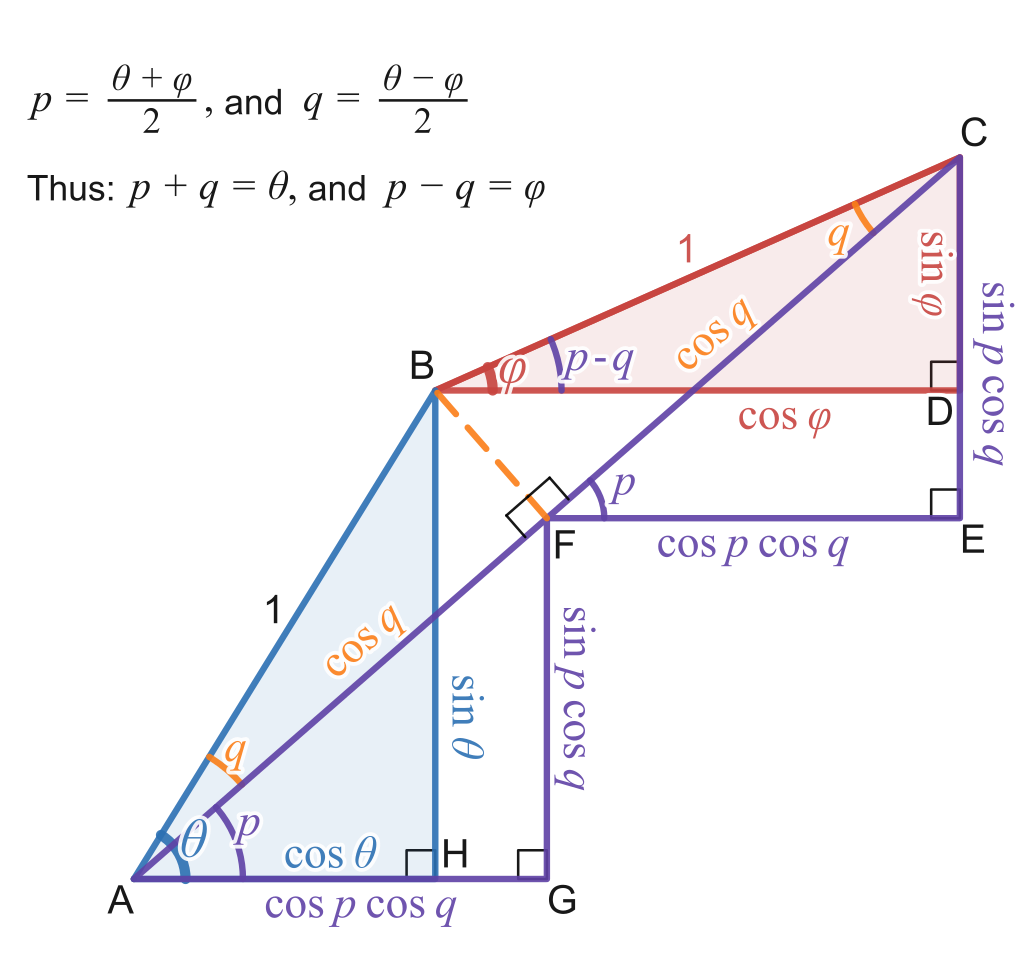
\includegraphics[width=0.5\textwidth]{figure/Diagram_illustrating_sum_to_product_identities_for_sine_and_cosine.png}
    \caption{Diagram illustrating sum to product identities for sine and cosine.}
\end{figure}

Figure \ref{fig:Diagram_illustrating_sum_to_product_identities_for_sine_and_cosine} 
illustrating sum-to-product identities for sine and cosine. 
The blue right-angled triangle has angle $\theta$ and the 
red right-angled triangle has angle $\varphi$. 
Both have a hypotenuse of length 1. Auxiliary angles, here called
$p$ and $q$, are constructed such that $p = (\theta + \varphi) / 2$ 
and $q = (\theta - \varphi) / 2$. Therefore, $\theta = p + q$
and $\varphi = p - q$.
This allows the two congruent purple-outline triangles
$AFG$ and $FCE$ to be constructed, 
each with hypotenuse $\cos q$ and angle $p$ at their base.
The sum of the heights of the red and blue triangles is
$\sin \theta + \sin \varphi$  and this is equal to 
twice the height of one purple triangle, 
i.e. $2 \sin p \cos q$. Writing $p$ and $q$ in that
equation in terms of $\theta$ and $\varphi$ yields 
a sum-to-product identity for sine:
\[
    \sin \theta + \sin \varphi = 2 \sin \dfrac{\theta + \varphi}{2} \cos \dfrac{\theta - \varphi}{2}
\]
Similarly, the sum of the widths of 
the red and blue triangles yields the corresponding identity for cosine.

